\documentclass[conference]{IEEEtran}
\IEEEoverridecommandlockouts
% The preceding line is only needed to identify funding in the first footnote. If that is unneeded, please comment it out.
\usepackage{cite}
\usepackage{amsmath,amssymb,amsfonts}
\usepackage{algorithmic}
\usepackage{graphicx}
\usepackage{textcomp}
\usepackage{xcolor}
\usepackage{tabularx}
\usepackage[colorlinks=true,urlcolor=black]{hyperref}
\graphicspath{ {./images/} }

\def\BibTeX{{\rm B\kern-.05em{\sc i\kern-.025em b}\kern-.08em
    T\kern-.1667em\lower.7ex\hbox{E}\kern-.125emX}}
\begin{document}

\makeatletter
\newcommand{\newlineauthors}{%
  \end{@IEEEauthorhalign}\hfill\mbox{}\par
  \mbox{}\hfill\begin{@IEEEauthorhalign}
}
\makeatother

\title{
    Tetris-AI - Triste\\
}


\author{
    \IEEEauthorblockN{MOLLY-MITTON Clément}
    \IEEEauthorblockA
    {
    \textit{College of Engineering} \\
    \textit{dept. Computer Science} \\
    Paris, France \\
    clement.mollymitton@gmail.com
    }
    
    \and
    
    \IEEEauthorblockN{BENDAVID OUYOUSSEF Sarah}
    \IEEEauthorblockA
    {
    \textit{College of Engineering} \\
    \textit{dept. Computer Science} \\
    Paris, France \\
    sarahbendavid@dartybox.com
    }
    
    \and
    
    \IEEEauthorblockN{HUBNER James}
    \IEEEauthorblockA
    {
    \textit{College of Arts and Sciences} \\
    \textit{dept. Criminal Justice} \\ 
    Alabama, United States \\
    jhub@uab.edu
    }
    
    \newlineauthors
    
    \IEEEauthorblockN{ARROUET LE BRIGNONEN Aubin}
    \IEEEauthorblockA
    {
    \textit{College of Engineering} \\
    \textit{dept. Computer Science} \\
    Paris, France \\
    aubin.arrouet$\_$le$\_$brignonen@edu.devinci.fr
    }
    
    \and
    
    \IEEEauthorblockN{MOBLEY Erin}
    \IEEEauthorblockA
    {
    \textit{College of Engineering} \\
    \textit{dept. Computer Science} \\
    Florida, United States\\
    erin.mobley@email.saintleo.edu
    }
}

\maketitle
\begin{abstract}
This project proposal aims to delve deeply into the game Tetris, focusing on two essential aspects. Firstly, it involves faithfully recreating the game Tetris and conducting an in-depth analysis of its functioning, design, and history. Secondly, this project seeks to develop an Artificial Intelligence (AI) capable of mastering Tetris to the extent of never losing.

The first part of the project entails a meticulous analysis of Tetris, breaking down its mechanics, design principles, and historical evolution. This analysis will shed light on the elements that have contributed to making Tetris an enduring cultural phenomenon and explain its consistent appeal.

The second component of the project is equally fascinating, involving the development of an Artificial Intelligence (AI) system that can achieve exceptional mastery of Tetris, avoiding losses altogether. By creating an AI capable of surpassing human-like strategic thinking and adaptability within the Tetris environment, we aim to push the boundaries of AI capabilities and explore potential applications of this technology in the realms of gaming, problem-solving, and AI research.
\end{abstract}

\section*{Role Assignements}

\begin{center}
\begin{tabular}{ | m{1.5cm} | m{1.2cm}| m{5cm} | } 
    \hline
    Roles & Name & Task description \\
    \hline
    User & 
    Erin & 
    - Proofreading documents: Erin, as a native English speaker, will review and edit project documents for language accuracy and clarity. She will ensure that the content is linguistically flawless.
    \newline- User Interface Development: Erin will be responsible for designing and developing the user interface, ensuring a user-friendly and visually appealing experience.\\
    \hline
    Customer & 
    Aubin & 
    - Resource Management: Aubin will oversee the allocation and utilization of project resources, ensuring efficient utilization of time and budget.\\
    
\end{tabular}
\end{center}

\begin{center}
\begin{tabular}{ | m{1.7cm} | m{1.2cm}| m{5cm} | }    
    &
    &
    - Support: Aubin will also have the mission of helping the various members in their tasks if necessary.\\
    \hline
    Software Developer & 
    Clément / James & 
    - Writing Code: James and Clément will be responsible for writing the code for the project, and implementing the game mechanics, AI algorithms, and system functionality.
    \newline- AI Development: They will also focus on creating and fine-tuning the artificial intelligence (AI) component of the project, allowing it to excel at playing Tetris.
    \newline- Documentation Assistance: In addition to coding, James and Clément will provide support in writing technical documentation, ensuring that the development process is well-documented. \\
    \hline
    Development Manager & 
    Sarah & 
    - Organizing the Project: Sarah will take charge of project organization, setting deadlines, scheduling meetings, and ensuring that project milestones are met.
    \newline- Coordination: She will facilitate communication and coordination among team members, ensuring that everyone is aligned and working effectively towards project goals.
    \newline- Technical Documentation: Sarah will be responsible for crafting technical documents that detail the project's architecture, design, and development processes.\\
    \hline
\end{tabular}
\end{center}



\section{Introduction}
\subsection*{Motivation}
Video games have always been a captivating realm of technological exploration and creativity, and among the most iconic titles in this industry, Tetris shines brightly. Created by Russian developer Alexey Pajitnov in 1984, Tetris has evolved into a global phenomenon, thanks to its addictively simple yet strategically rich gameplay. This puzzle game has enthralled entire generations of gamers, delivering a timeless gaming experience.

This is precisely why our interest was piqued by Tetris. While Tetris's rule set is very simple the multitude of strategies one can employ to strive for the highest score is particularly fascinating. Naturally, some strategies prove more effective than others. Given Tetris' universal recognition, we found it compelling to create an AI capable of playing the game endlessly while employing the most advanced strategies. To realize this project, we must rebuild Tetris from the ground up and design a sophisticated AI that excels in the game.

Developing an AI with the ability to indefinitely succeed at playing Tetris presents a complex problem-solving challenge. It necessitates critical thinking, the creation of innovative strategies, and the optimization of algorithms for maximum efficiency. Through this endeavor, we will not only employ and apply theoretical AI concepts but also enhance our software engineering skills.

\subsection*{Problem statement}
The objective of Tetris is simple, Match the tiles to form a line so that it clears space in the board. Tetris was designed to be endless, However, there comes a point in the game where the player cannot continue. This happens when enough uncleared rows build up and there is no room left on the board to add the next generated game piece (tetrominoes).

With the inclusion of Artificial Intelligence, could the games be pushed to their limits, and a truly endless game of Tetris be achieved? How can we design a Tetris AI that not only places the tetrominoes efficiently but also can adjust to the gameplay mechanics of ever-increasing gravity with the randomness of block combinations, while still taking the player’s inputs into account? The AI should still mimic the decision-making done by humans once it is aware of the upcoming tetrominoes, checking for the best placement, and executing its decision to allow the game to continue for as long as possible.

\subsection*{Research on any related software}
Several AIs have been implemented in Tetris to cover all the different ways of playing the game. Indeed, Tetris has been implemented with different AIs over the years for several purposes: creating its computer opponents or creating its own recommendation system. 
Several videos have been posted on Youtube presenting AIs that could play Tetris, some indefinitely:
\subsection{Code Bullet}
The AI coded by Code Bullet\cite{b1} was reported as being the first AI to beat the human world record. It managed to get a score of around 15,000 points, he also said if he continued training and improving it, the AI could possibly become invincible.
\subsection{StackRabbit}
The AI coded by Greg Cannon\cite{b2} managed to break Tetris NES. It broke the game because when the game is played on the console, scores that are too high can cause the game to crash because of the way the score is calculated. After reaching a score of 102 million, the game crashed and so the AI broke the game and thus could be considered invincible.
\subsection{Github}
Making a Tetris-solving AI is a typical project for students, people who want to learn using AIs, and simply people who enjoy the game. A lot of people then posted their projects on Git Hub\cite{b3}, consequently, there is a huge amount of GitHub projects for a Tetris AI.

\section{Requirements}
\section*{Creation of TETRIS}
\subsection{Game Grid}
Create a graphical representation of the game grid using appropriate rendering techniques, clearly displaying the current state of tetrominoes and placed blocks.
\subsection{Tetromino Generation}
The tetromino generation will use a random generation algorithm. We would like, if possible, to use the exact random generation algorithm that the original Tetris uses to keep the maximum amount of fidelity possible.
\subsection{Movement and Rotation}
Development functions to handle the movement (left, right, down) and rotation of tetrominoes based on player input. Tetris also has more advanced mechanics in which when the player rotates the tetromino, this one stays in place and doesn’t descend, this function should also be developed.
\subsection{Controls}
The control system in a Tetris game is a critical component of ensuring an enjoyable and engaging player experience. It should offer responsiveness and intuitiveness, allowing players to manipulate Tetris pieces with precision.
\subsection{Collision Detection}
Implement collision detection algorithms to determine when a tetromino reaches the limit of the grid or collides with another tetromino, triggering actions like line clearing.
\subsection{Line Clearing}
Implement the logic to detect and clear complete lines when a tetromino fills a row, adjusting the game grid and influencing the score.
\subsection{Scoring System}
Design and implement a scoring system that rewards points based on the number of lines cleared simultaneously (single, double, triple, or Tetris) and the level of the game.
\subsection{Level and Game speed}
The game speed of Tetris increases when the score increases. The game speed of Tetris increases by steps rather than linearly and is capped after reaching a certain score, the precise speeds and the scores at which they are used in the game should be the same as in the original Tetris.
\subsection{Game Over}
Define conditions for ending the game, typically when the game grid becomes too congested to accommodate a new piece. Display a game over screen that shows the player's final score and provides an option to restart the game.
\subsection{HUD Elements}
Design and integrate HUD elements, including score display, level indicator, and upcoming tetromino preview, providing essential information to the player during gameplay. For the AI, these functions should also be inputs that are directly provided to the AI so it can play without having to use the graphical interface. This interface is simply used for the human users of the game.

\section*{Creation of the AI}
\subsection{Data Collection}
The AI system needs access to a comprehensive dataset of Tetri's gameplays from which it can learn. This dataset should encompass a variety of game scenarios, including different starting positions, levels, and player actions.
\subsection{Input Processing}
The AI should possess the ability to process the current game state, which includes the current Tetrimino, the matrix of filled blocks, and the current score.
\subsection{Strategy Development}
The AI system must develop a strategic approach to decision-making regarding the placement of Tetriminos. This strategy should take into account various factors such as maximizing score, clearing lines, avoiding stacking blocks, and ensuring long-term success.
\subsection{Adaptability}
The AI system must be designed to adapt to different levels of difficulty and game speeds. This adaptability ensures that the AI can effectively handle various game scenarios and continue to perform well as the game progresses.
\newline
\newline
By fulfilling these general requirements, it is possible to design and develop an AI system that can efficiently learn and play Tetris. However, it is important to note that the AI will require continuous refinement, debugging, and iteration to improve its performance and ensure its success in various game scenarios.


\section{Development environment}
\subsection{Choice of software development platform}

\subsection*{Software platform}

Our project is being carried out on the Windows software platform. Windows is compatible with a wide range of Python development tools, including VisualStudio Code and IDLE, which make it easier to debug code. Windows also supports the Python libraries and frameworks commonly used for AI development, including Pygame\cite{b4} and PyTorch\cite{b5}. Our project is a game, which needs to be manipulated by as many people as possible. Our aim is to be able to share it with users. Windows seemed the best choice, because it supports a wide variety of hardware configurations. This means that if we develop our game, it will be compatible on a wide range of computers. As we are all familiar with the Windows environment, it was an obvious choice for us.




\subsection*{Programming language}

We decided to create our game in Python, mainly for its simplicity and readability, which makes it easier to create Tetris and implement the AI. Python is a rich computer language, full of libraries that make game creation easier. It has a vast collection of frameworks that are useful for game development (notably Pygame\cite{b4}). Python has also become a programming language that is frequently used to create AI (thanks in particular to the Sickit-learn and PyTorch libraries\cite{b5}). Because Python is an interpretive language, we can develop, test and iterate quickly. The debugging tools are effective and, being familiar with the language, we can move forward more quickly and correct our mistakes. 
That's why Python seemed to be the best choice. 

\subsection*{Development Environment}
The project will be developped using Spyder, which is a free and open source development environment for python coding.  It features a unique combination of the advanced editing, analysis, debugging, and profiling functionality of a comprehensive development tool with the data exploration, interactive execution, deep inspection, and beautiful visualization capabilities of a scientific package. In terms of computer ressources, we have  access to five laptops, including two gaming laptops with advanced consumer available CPUs which could be helpful to the free training of the AI.

\subsection*{Cost estimation }
By creating our code from scratch in Python, the project will cost nearly nothing. All we need to do is download Python (a programming language that can be downloaded free of charge). By downloading Python, various libraries can be installed, also free of charge. These are the ones we will be using to create our AI. Furthermore, to train our AI, we will likely use AWS, which costs almost nothing when we select certain specific configurations.


\subsection{Software in use}

\subsection*{Teams}
Teams is an important tool for organizing our project. It allows us to assign tasks to each team member on a weekly basis and track the progress of these tasks. It also serves as the platform for our video conferences. Additionally, Teams facilitates file sharing, real-time document collaboration, and link sharing within our project channel.
\subsection*{KakaoTalk}
KakaoTalk will be our primary tool for quick and spontaneous communication. Through our dedicated channel, team members can keep each other informed about tasks, their status, and deadlines. It provides an ideal platform for asking questions and staying updated.
\subsection*{LaTex}
LaTeX serves as our primary document creation tool, enhancing the efficiency and quality of our project documentation. It excels in formatting, versatility, and facilitating collaboration. It ensures clear and standardized formatting, allows easy inclusion of complex elements, and simplifies version management and collaboration in our project.
\subsection*{Overleaf}
To meet our project requirements, we have adopted Overleaf as a central platform for creating well-organized, scientific reports detailing the progress and completion of our project. Overleaf empowers us to work collaboratively on LaTeX documents, facilitating seamless and efficient document creation, editing, and revision.
\subsection*{GitHub}
GitHub is a key tool in our project's software toolkit, streamlining version control, collaborative development, and project management. It serves as a web-based platform for hosting project source code, ensuring accessibility to all team members. Integration with Git simplifies remote storage management, while enabling seamless collaboration in our project. It facilitates concurrent work on different project aspects and eases code review and integration to maintain software quality.
\subsection*{PyGame}
Pygame\cite{b4} is a library ideally suited for 2D games, making it a perfect choice for implementing Tetris. It offers a set of tools for managing 2D graphics, such as creating a game window, rendering Tetris pieces, and handling player input. Due to its versatility and simplicity, Pygame is a wise choice for developing Tetris.
\subsection*{Pytorch}
Our Tetris game will also be played by an AI, developed using Pytorch\cite{b5}. Pytorch is particularly well-suited for reinforcement learning algorithms, which are essential for training the AI to play Tetris. Pytorch can also simulate the game environment and allow the AI to interact autonomously while learning from its experiences. It enables the AI to generate actions, such as moving and rotating pieces, using a neural network. Importantly, the AI can continue learning in real time without interrupting the game, making Pytorch a complementary tool to Pygame, which provides the game interface and piece manipulation capabilities.

\subsection{Task distribution}


\section{Specifications}

\section*{Creation of TETRIS}
\subsection{Game Grid}
The game grid is represented as a two-dimensional data structure, specifically, a list of lists of integers. In this grid, the value 0 denotes an empty cell, while the value 1 signifies a cell that is occupied by a block. Additionally, a secondary matrix is employed to store the requisite color information for rendering the game grid.
\subsection{Tetromino Generation}
Each game piece consists of three key attributes: a shape, a color, and its position coordinates within the grid. To ensure diversity in the generation of these pieces, we employ Python's "random"\cite{b6} library, which allows us to select randomly the colors and shapes.
\subsection{Movement and Rotation}
Facilitating player control over the game pieces involves verifying the validity of the requested movements and executing them accordingly. For horizontal (right and left) and vertical (down) movements, the piece's coordinates are simply updated in the respective direction. When it comes to rotation, we perform a 90-degree rotation of the matrix representing the piece's shape.
\subsection{Controls}
Players can interact with the game pieces using the arrow keys: left, right, and down for lateral movement, and the up key for a 90-degree rotation.
\subsection{Collision Detection}
Collision detection plays a critical role in gameplay by ensuring the legality of movements. We incorporate conditions within the verification method of the grid to ensure that the coordinates stay within the grid boundaries and do not conflict with cells already occupied by other pieces.
\subsection{Line Clearing}
To clear complete lines, we will simply check if an entire row of the board is composed entirely of 1's. In that case, we will remove that row from the list of lists and add a new empty row to the beginning of the grid.
To detect and remove completed lines, we simply examine each row of the grid to ascertain if it consists entirely of 1's. In such cases, we remove that row from the list of lists and append an empty row at the top of the grid.
\subsection{Scoring System}
Scoring in the game is incrementally updated each time the board lines are cleared. Whenever a line is successfully cleared, the player's score is increased accordingly.
\subsection{Level and Game speed}
Controlling the pace of the game is achieved by adjusting the frequency at which tetrominos descend. By manipulating the clock, we can reduce the time interval between piece drops, effectively increasing the game's speed as the player progresses to higher levels.
\subsection{Game Over}
The game over condition is triggered when it becomes impossible to place a newly generated piece due to the presence of obstructing pieces. A dedicated function will be implemented to detect and respond to this scenario.
\subsection{HUD Elements}
For rendering various game elements, the "pygame"\cite{b4} library is employed. This library enables the creation of a customized game window that can be tailored to present the game in a visually appealing and informative manner.
\begin{figure}[h]
    \centering
    \fbox{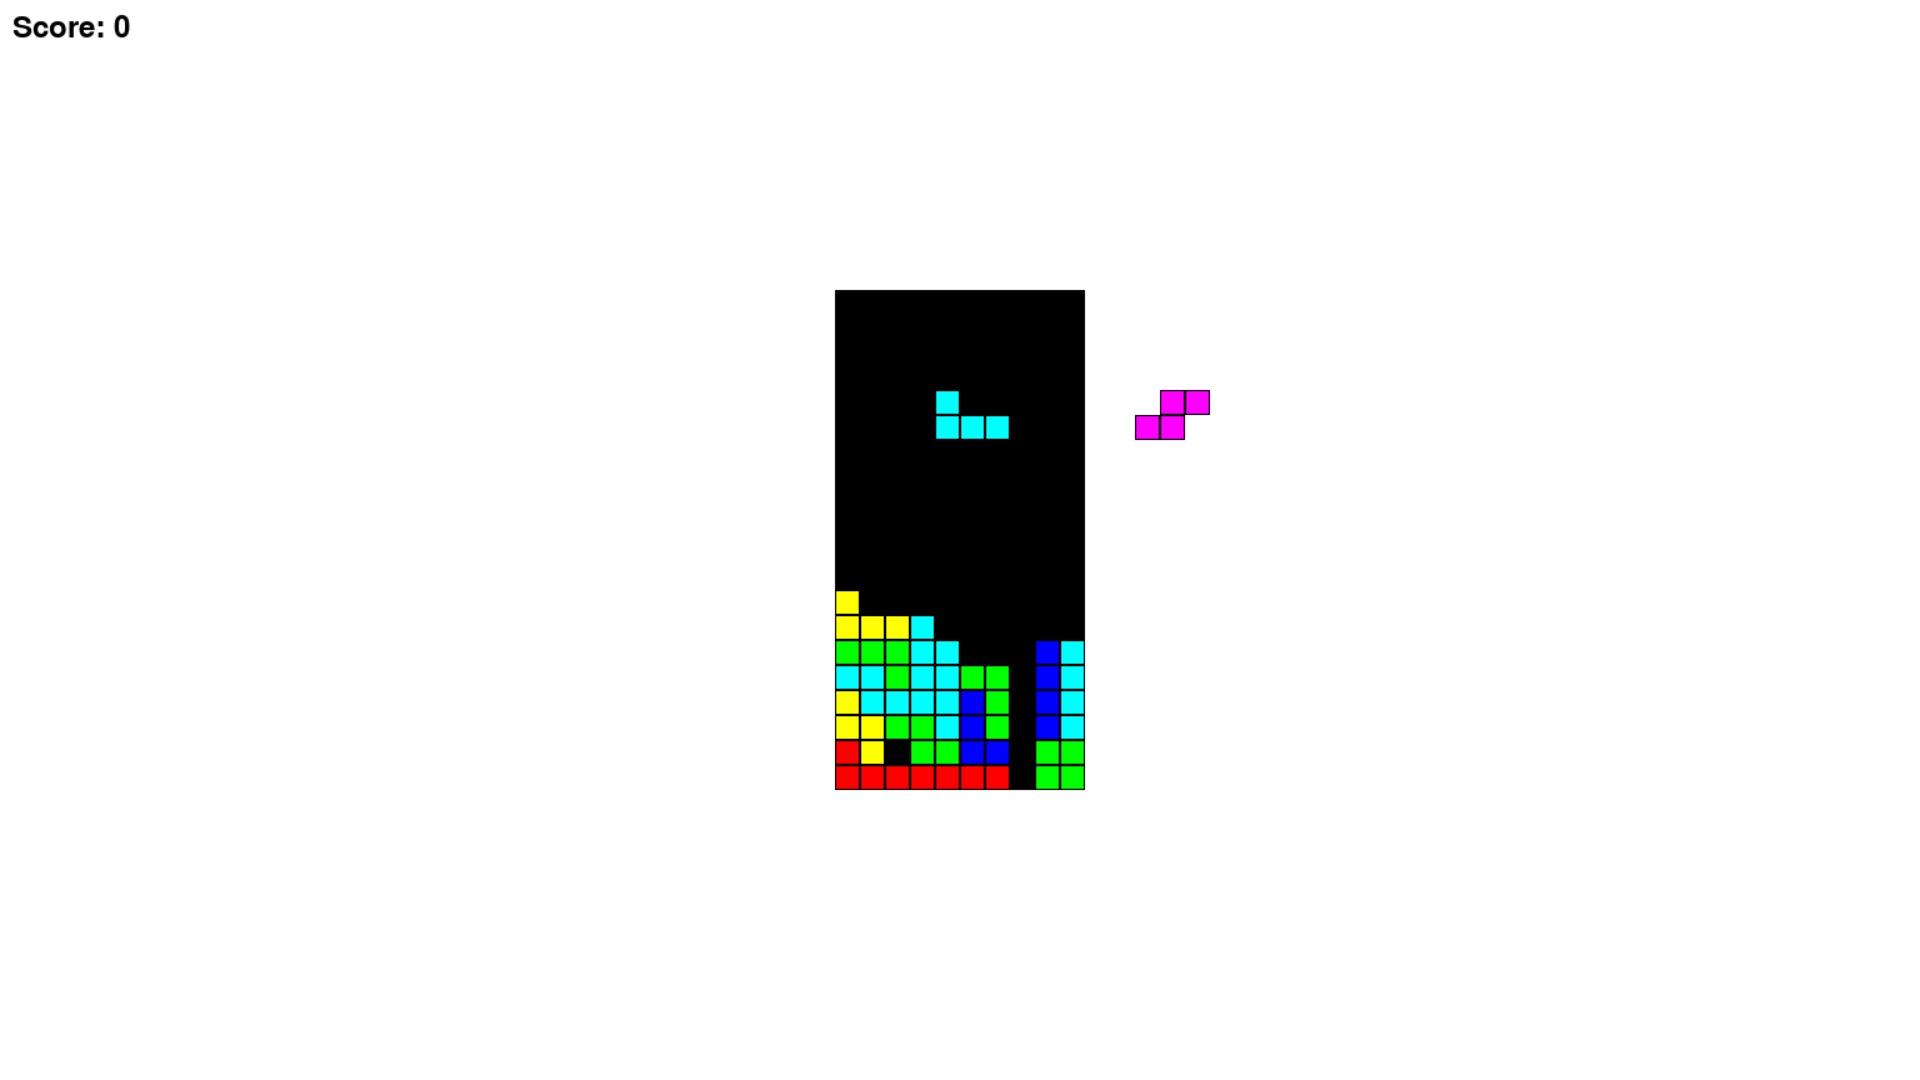
\includegraphics[scale=0.13]{Specification_HUDElements}}
    \caption{Our first display of Tetris}
    \label{fig:Display}
\end{figure}

\section*{Creation of the AI}

\subsection{Data Collection}
In order to train the AI for playing Tetris, we need to collect a dataset of game states and corresponding actions. This involves recording the current state of the game grid, including the positions and shapes of the tetrominoes, as well as the potential actions that can be taken. The dataset should also include the corresponding action that the AI should have taken in that state. This data can be collected by simulating gameplay with human players or through self-play.
\subsection{Input Processing}
Once the dataset is collected, we need to process the input data to prepare it for training the AI model. This involves converting the game state information, such as the positions of the tetrominoes and the game grid, into a suitable format that can be fed into the AI model. The input data may also need to be normalized or preprocessed to ensure consistent and meaningful representations.
\subsection{Strategy Development}
The AI needs to develop a strategy for playing Tetris effectively. This involves training a machine learning model, using the collected dataset. The model should be trained to predict the best action to take given a particular game state.
\subsection{Adaptability}
To make the AI adaptable, it should be able to learn and improve its strategies over time. This can be achieved by continuously updating and retraining the AI model with new data as more gameplay is recorded. The model should be able to generalize its knowledge and adjust its strategies based on the changing game dynamics and patterns observed in the data. This adaptability will allow the AI to become increasingly proficient at playing Tetris.

\clearpage
\section{Architecture Design Implementation}
\subsection{Overall Architecture}

\begin{figure}[h]
    \centering
    \fbox{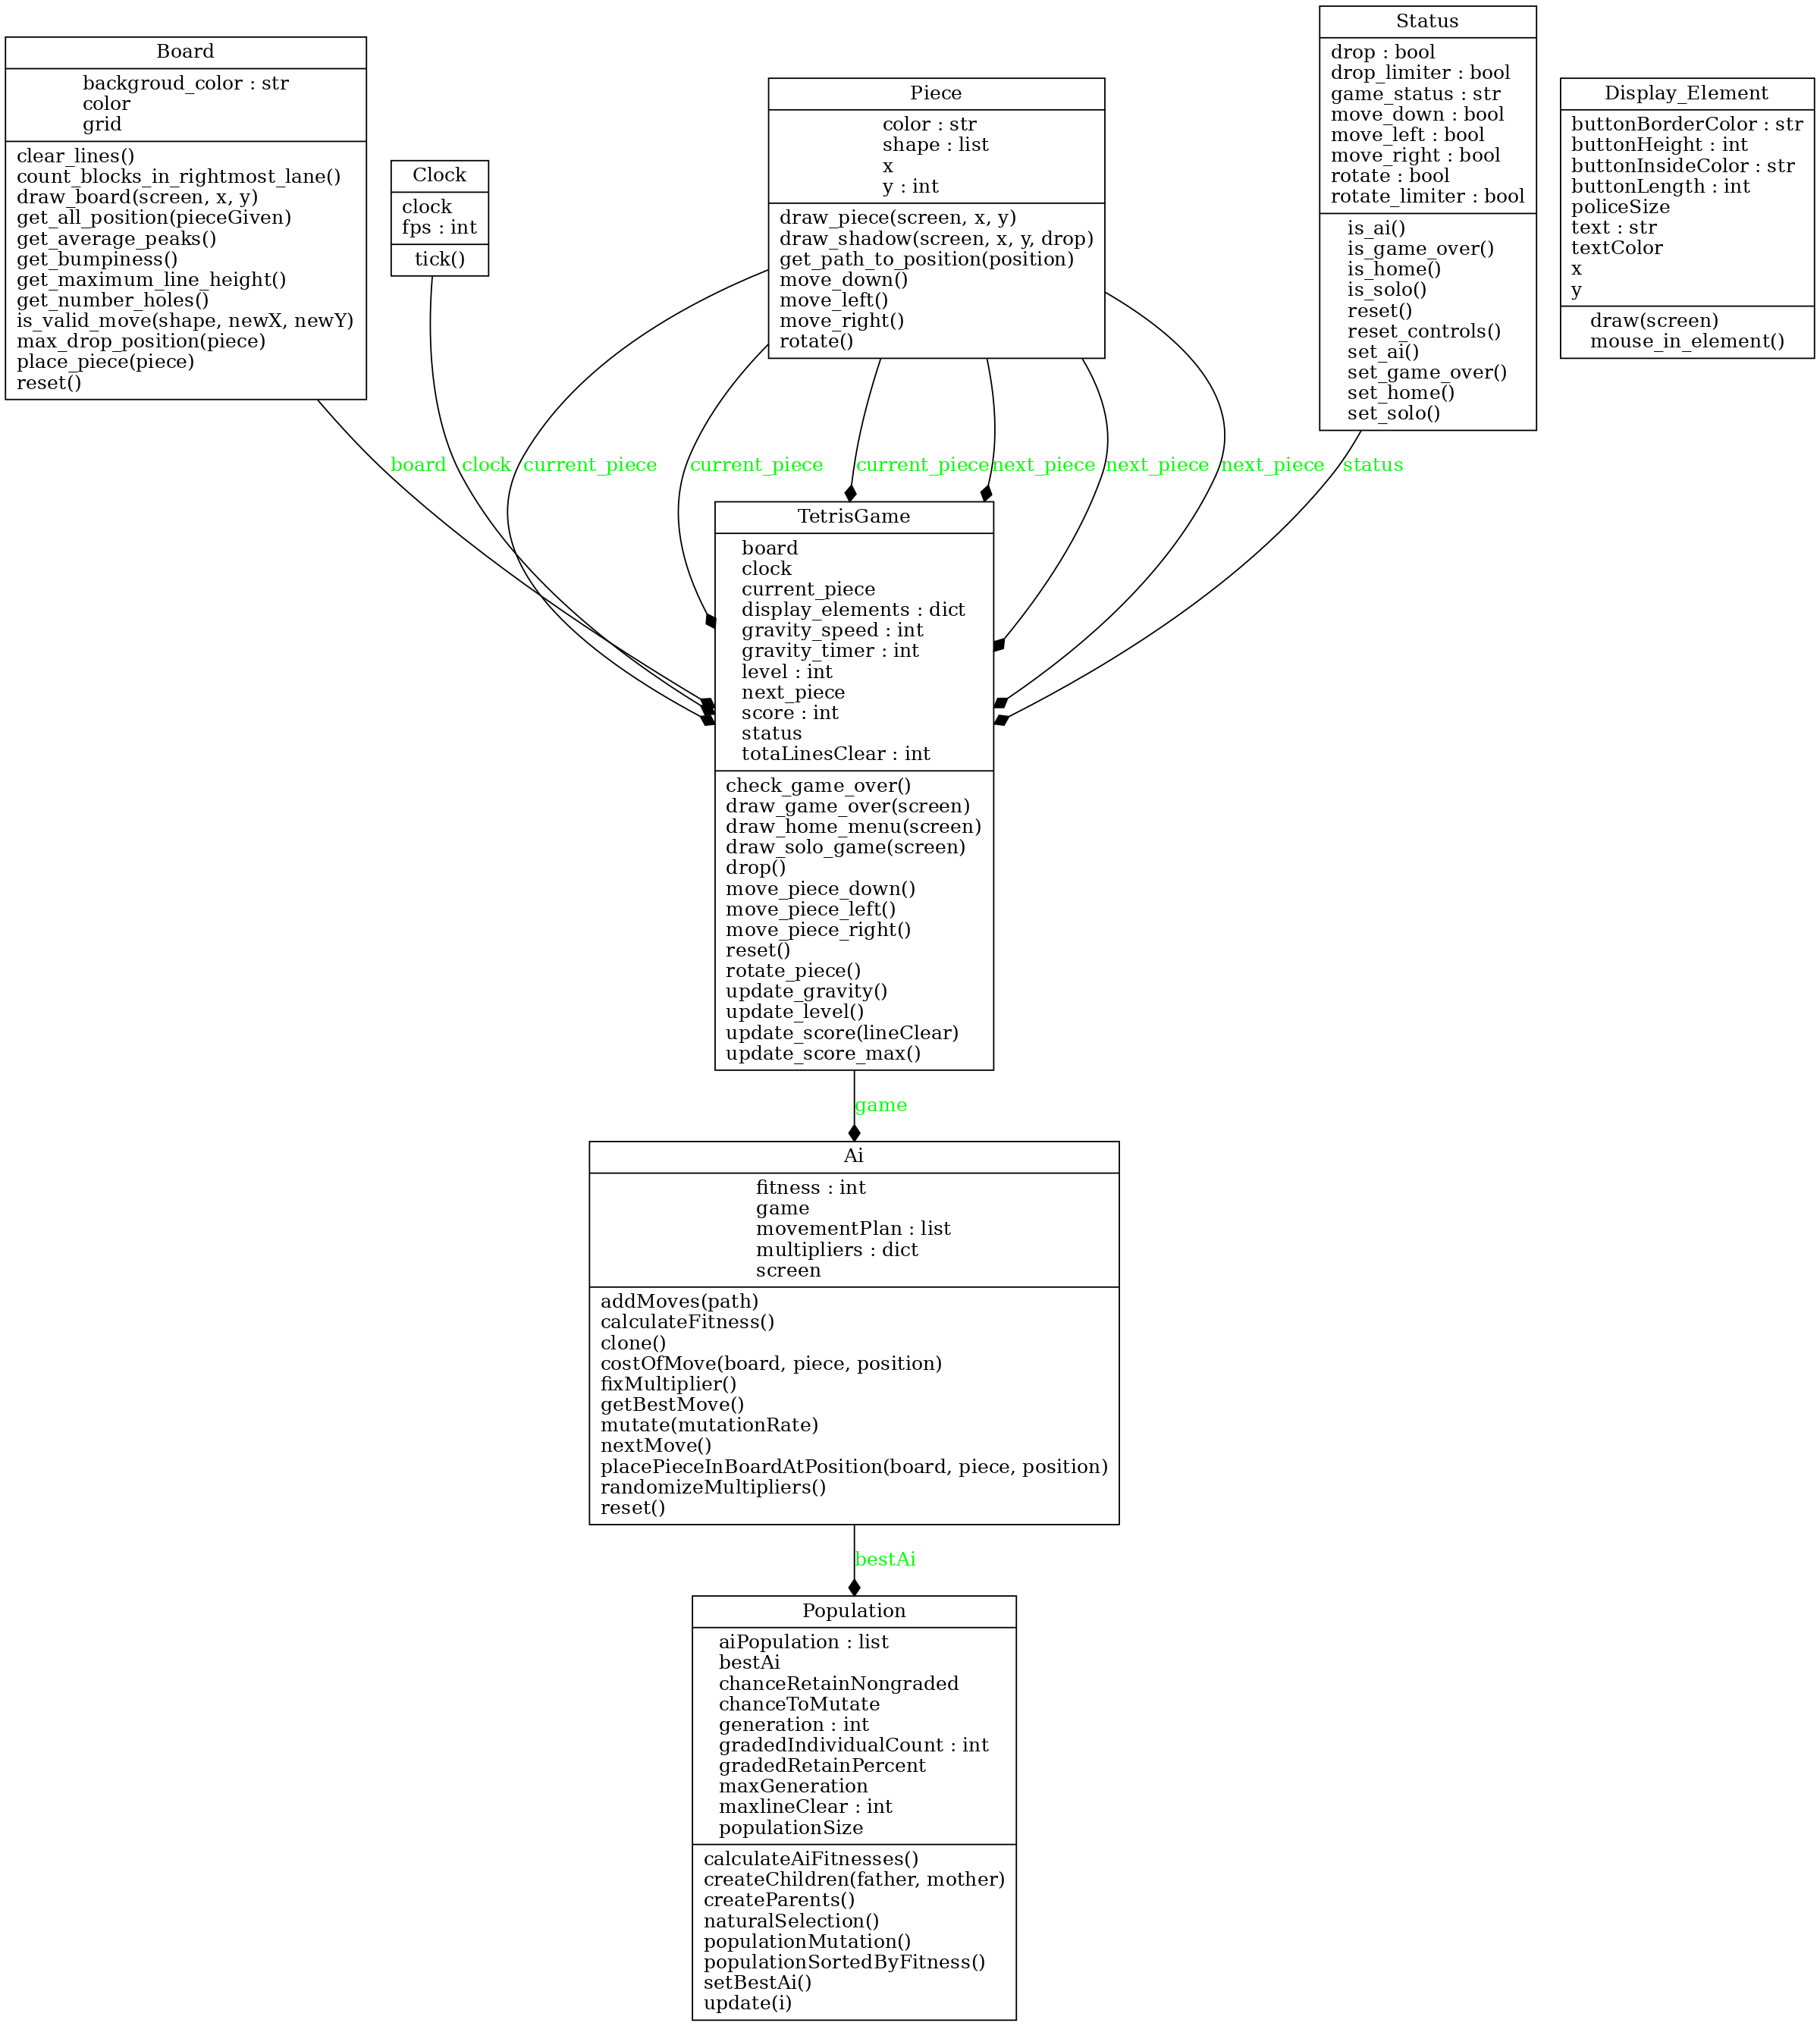
\includegraphics[scale=0.211]{images/triste_uml.png}}
    \caption{UML}
    \label{fig:Display}
\end{figure}
\clearpage

\subsection{Directory organization}

\begin{center}
\begin{tabular}{  | m{1.3cm} | m{1.7cm} | m{4.7cm} | } 
    \hline
     Directory & Files name & Description \\
    \hline
    Tetris-AI & 
    tetrisgame.py & 
    - The purpose of this code is to create our Tetris game base. It uses nearly all the  class in the other py files to create a Tetris game. The current piece is managed using methods such as move$\_$piece$\_$left, move$\_$piece$\_$right, move$\_$piece$\_$down  rotate$\_$piece and drop methods
    \newline- The class updates the score with update$\_$score and the level with update$\_$level according to the lines cleared. The graphical display, including the home and end of game screens, is handled by the draw$\_$home$\_$menu, draw$\_$solo$\_$game and draw$\_$game$\_$over methods using the Pygame\cite{b4} library. \\
     \hline
     Tetris-AI &
    piece.py & 
    - The Piece code defines a Piece class to represent the pieces in the Tetris game. Each instance of the class is a piece with a random shape, a corresponding colour, and x and y coordinates for its position. This code can be used to direct the part to the left, right or bottom, to rotate it, and to draw the part and its 'shadow' on the screen. Moreover The get$\_$pathto$\_$position method returns the list of movements necessary to move the piece to a specific position.\\
     \hline
    Tetris-AI & 
    population.py &
    - The population code implements a genetic algorithm to evolve an AI population in Tetris. It promotes the reproduction of the best adapted individuals. The Population class manages the initial creation of the population, natural selection, mutation and the creation of new generations of AIs.  
     
\end{tabular}
\end{center}


\begin{center}
\begin{tabular}{ | m{1.3cm} | m{1.7cm} | m{4.7cm} | } 

    Tetris-AI & 
    population.py &
     The update function is used to progress each individual through the game simulation, calculateAiFitnesses to evaluate the performance of each AI, naturalSelection to carry out natural selection.\\
      
    \hline
    Tetris-AI & 
    training.py & 
    - The aim of the training is to train an AI capable of maximising the number of lines deleted in the game Tetris. It uses the Population class by instantiating it, then iterating over the generations, updating the individuals and performing natural selection.\\
     \hline
     Tetris-AI & 
    status.py & 
    - The Status class in Python is a status handler for the Tetris game. It includes methods such as set$\_$game$\_$over, set$\_$home, set$\_$solo, set$\_$ai to change the status of the game. The is$\_$home, is$\_$game$\_$over, is$\_$solo, and is$\_$ai functions are used to check the current state of the game. The class also provides reset methods, including reset$\_$controls to reset controls, and reset to reset the entire state of the game.\\
     \hline
    Tetris-AI & 
    main.py & 
    - This code uses the Pygame library to implement the Tetris game, integrating essential Pygame functions such as keyboard/mouse event management with pygame.event.get() and display updating with pygame.display.update(). Tetris features are managed by the class instance of tetrisgame. \\
    \hline
    Tetris-AI & 
    display.py & 
    - This code implements a class called Display$\_$Element, which creates graphical elements, such as buttons, for the Tetris user interface. Moreover this class contain methods that are really useful for the user action detection like the  mouse$\_$in$\_$element(), which checks whether the mouse is on the element.\\

\end{tabular}
\end{center}


\begin{center}
\begin{tabular}{| m{1.3cm} | m{1.7cm} | m{4.7cm} | } 

    Tetris-AI & 
    constants.py &
    - This code defines useful constants for the game, including the dimensions of the grid (gridWidth and gridHeight), the size of each cell (cellSize), the frame rate (fps), and the maximum possible score (maxscore). It has also a lists the different shapes of Tetris pieces with their representation in matrices of 1 and 0, as well as the colours associated with each shape (color$\_$per$\_$shape). Moreover, include colour dictionary (colors) to represent the different colours used in the game.
    \newline-Finally it as a maxScore line for the save of the best score. All these element necessary to ensure that the game is consistent and easy to maintain and having them in one file is pratical. \\
    \hline
    Tetris-AI & 
    clock.py & 
    - This code defines a Clock class in the Pygame module. The class is used to manage time and updates at a specific rate of frames per second (fps). In the constructor ($\_$$\_$init$\_$$\_$), a pygame.time.Clock object is initialised, and the constant fps from the constant module is assigned to the fps attribute of the class. The tick method is defined to obtain the time elapsed since the last call to the tick function and maintain the defined frame rate. This class is useful for controlling the speed of the game, and ensuring that it runs at a constant rate. \\
     \hline
     Tetris-AI & 
    board.py & 
    - The Board code uses the Pygame module. It tests the validity of piece movements with is$\_$valid$\_$move, place$\_$piece to place a piece on the board, clear$\_$lines to clear complete lines.
    - Also max$\_$drop$\_$position to determine the maximum drop position of a piece, and methods evaluating various aspects of the grid such as the height of peaks (get$\_$average$\_$peaks), irregularity (get$\_$bumpiness), number of holes (get$\_$number$\_$holes), and so on. \\

\end{tabular}
\end{center}


\begin{center}
\begin{tabular}{ | m{1.3cm} | m{1.7cm} | m{4.7cm} | } 
    Tetris-AI & 
    ai.py & 
    -  AI functions include calculateFitness to evaluate the AI's performance, getBestMove to determine the best possible move, mutate to introduce mutations into the evaluation multipliers, and clone to create a copy of the AI. The AI uses multipliers to evaluate moves according to various criteria, such as the number of holes, the irregularity of the board, the number of lines erased, and so on. \\
    \hline
\end{tabular}
\end{center}

\subsection{Module 1 : Main}
The purpose of main is to provide the user with the ability to choose between a solo game, the AI game and exiting the program. Moreover, when Solo game is selected, main will check the key inputs of the player and assign the correct actions to the Tetris game. Finally, when the player loses, it shows the game over screen. If AI game is selected, main will create a tetris game and then use the AI class to play it. For each move, main calls getBestMove function from the AI class to determine the best move. After the best move is determined, main will go to the next move. This is repeated untill game over.
Main's components are: display (the display of the game),  game (which is an instance of the Tetris game class), ai (which is an instance of the Ai class) and running, which is used to check if the user wants to exit the program, it is initialized as true at the start)

\subsection{Module 2 : Constants}
As it's name suggests, constants is a file in which all of the global constants necessary to the well functioning of the program are stored. Those include constants for the board such as the grid width and height and cell size. It also stores the frames per seconds, the best score ever on the game, the different shapes of the tetrominos and the different colors of the shapes and all the color useful for the display of the game.

\subsection{Module 3 : Clock}
The clock class is simply used to act as the clock in the game, adapting it's ticks to the fps variable stored in constants

\subsection{Module 4 : Board}
Board has two main variables, the grid which stores the different cells that are filled by  placed tetrominos, and the colour matrix which stores the colours of each cell for the display of it to the player/ observer.
Board has several functions that are used both by solo players and the AI, those functions are used in piece movements and placement, such as verifying if a movement is valid (not out of bounds or clipping with already placed tetrominos), placing a piece on the board, clearing completed lines. Also, the function draw$\_$board manages the display of the board, and reset$\_$board resets it
Moreover, Board also has specific functions for the AI. In those, some functions help to extract some data from the board for the AI to use, such as  the height of the highest column, the average height of the columns, the bumpiness, the number of holes in the structure of placed tetrominos and finally the number of filled cells in the right column (this helps determine the chances of making a Tetris). Also, the function get$\_$all$\_$positions will return all of the possible positions in which a piece can be placed on the board in the current configuration, this function will allow the AI to determine the best move according to it's model.
All of the functions of board are written here because of their strong reliance on using data from the grid of the game to display the game, check the validity of moves, and extract useful data for the AI

\subsection{Module 5 : Piece}
Piece is initialized by creating a random shape from the shapes array in constants. This piece can then be used in the Tetris game. The piece class has functions dedicated to movement (right, left, down, rotate), display of the piece and it's shadow on the drop position right under it's current position, and finally it has the get$\_$path$\_$to$\_$positon which is useful for the AI to write the necessary movement the piece need to do to attain a specific position on the board.

\subsection{Module 6 : Display}
Display is a class used to make the tools that are used to display information to the rest of the program or button. This class was principally created to facilitate the creation of display element and also the detection of the user behavior for each element created. 

\subsection{Module 7 : Status}
Status stores different data on the status of the game. The variable game$\_$status can be "Home" for the home screen, "solo" for the solo game, "Ai" for the AI game and finally "game over. Status also stores data relative to the movement of pieces such as if it's moving right, left, down, rotating and dropping. Finally it has a function to reset the controls and to resets itself entirely.

\subsection{Module 8 : Tetris}
Tetris game stores the main tools used to make a Tetris game work. It imports the constants grid width,grid height,cellSize and maxscore. It also imports an instance of Board, Clock, Piece, Status and Display$\_$Element. With those, it also has specific variables such as the current and next pieces to be played, the score, the level, the gravity (speed at which the pieces fall), the game status and the display elements associated with that status. First Tetris is used to display all of the home screen (Home solo button, home ai button, home exit button, best score, etc), and does similarly with the game over screen and the in game screen. Then it has functions dedicated to game controls for moving left, right, and rotate while checking that the moves are valid. It also checks for game overs. Finally, it also has tools to update the game, such as updating the levels and gravity (speed at which the piece falls), updating the score and displaying those updates on the in game screen.

\subsection{Module 9 : AI}
The AI class is the main tool to use an AI according to a model to play Tetris. The AI class is not only used to play the game, but also provides useful data for the training using a genetics algorithm.
The AI class imports TetrisGame. In terms of variables, AI has the current game being played for the instance of TetrisGame, multipliers for the different data collected, the fitness of the AI (used in training), the movement plan (the list of movements to do in order in the game) and a screen. In terms of functions, AI has two functions for the multipliers of data, one is fixed and predermined for the best  multipliers currently found, and the other is to set the multipliers randomly. The calculatFitness function calculates how good the AI is depending on it's best score. The nextMove function applies the first move (moving right, left, rotating or dropping)  and switches to the next one to do. The placeInBoardAtPosition function directly places a piece at a specific position. The costOfMove function calculates how good a specific move is for the AI depending on the multipliers that were previously defined. getBestMove chooses the best move amongst all of the possible moves in the current game configuration. Then AI has two functions for the genetic algorithm part: mutate and clone. Finally it has a reset function.

\subsection{Module 10 : Population}
The population class has for goal to manage a population of AIs through different generations, it creates generations and then has functions to make them evolve through time with a genetics algorithm.
Population imports AI. It has several class variables, those are populationSize, maxGeneration (maximum number of generations), chanceToMutate, gradedRetainPercent (the percentage of the best AIs to retain), chanceRetainNongraded (chance to retain bad AIs), screen and then AI population which is a list of AIs.
In terms of functions, population has one for updating the AI, calculating the overall fitness for all AIs, sorting the population based on fitness, and selecting the best AI in the generation. Moreover population has functions for keeping the AIs (the parents) and creating offspring to complete the population (createParents and createChildren). Additionally, Population has functions to potentially mutate the population and the function responsible for the entire natural selection process.

\subsection{Module 11 : Training}
The training.py file can be executed to train the AI. It uses population.py to manage the different generations and use the genetics algorithm. In training you can set the parameters you desire for the training in the following variables: populationSize, maxGeneration, chanceToMutate, gradedRetainPercent, chanceRetainNongraded
While the number of generations or the chosen "win" criteria (for us it was clearing 1000 lines) isn't completed it repeats the following operation: executing a population generation through using multithreading (which was faster than multiprocessing for our case) and applying the genetics algorithm to create a new generation. It also prints the max number of lines cleared by an AI to check the progress made during each generation.
Finally, it prints the generation at which the "win" criteria was completed and shows the time it took.

\section{Use Cases}
\begin{enumerate}
    \item Game Launch and Menu Screen: \\
When the user launches the game, they will be presented with the following Menu Screen. From this Screen, the user can select to run the Tetris game in Solo Mode, AI Mode or Exit the game.
\begin{figure}[htbp]
\centering
    \fbox{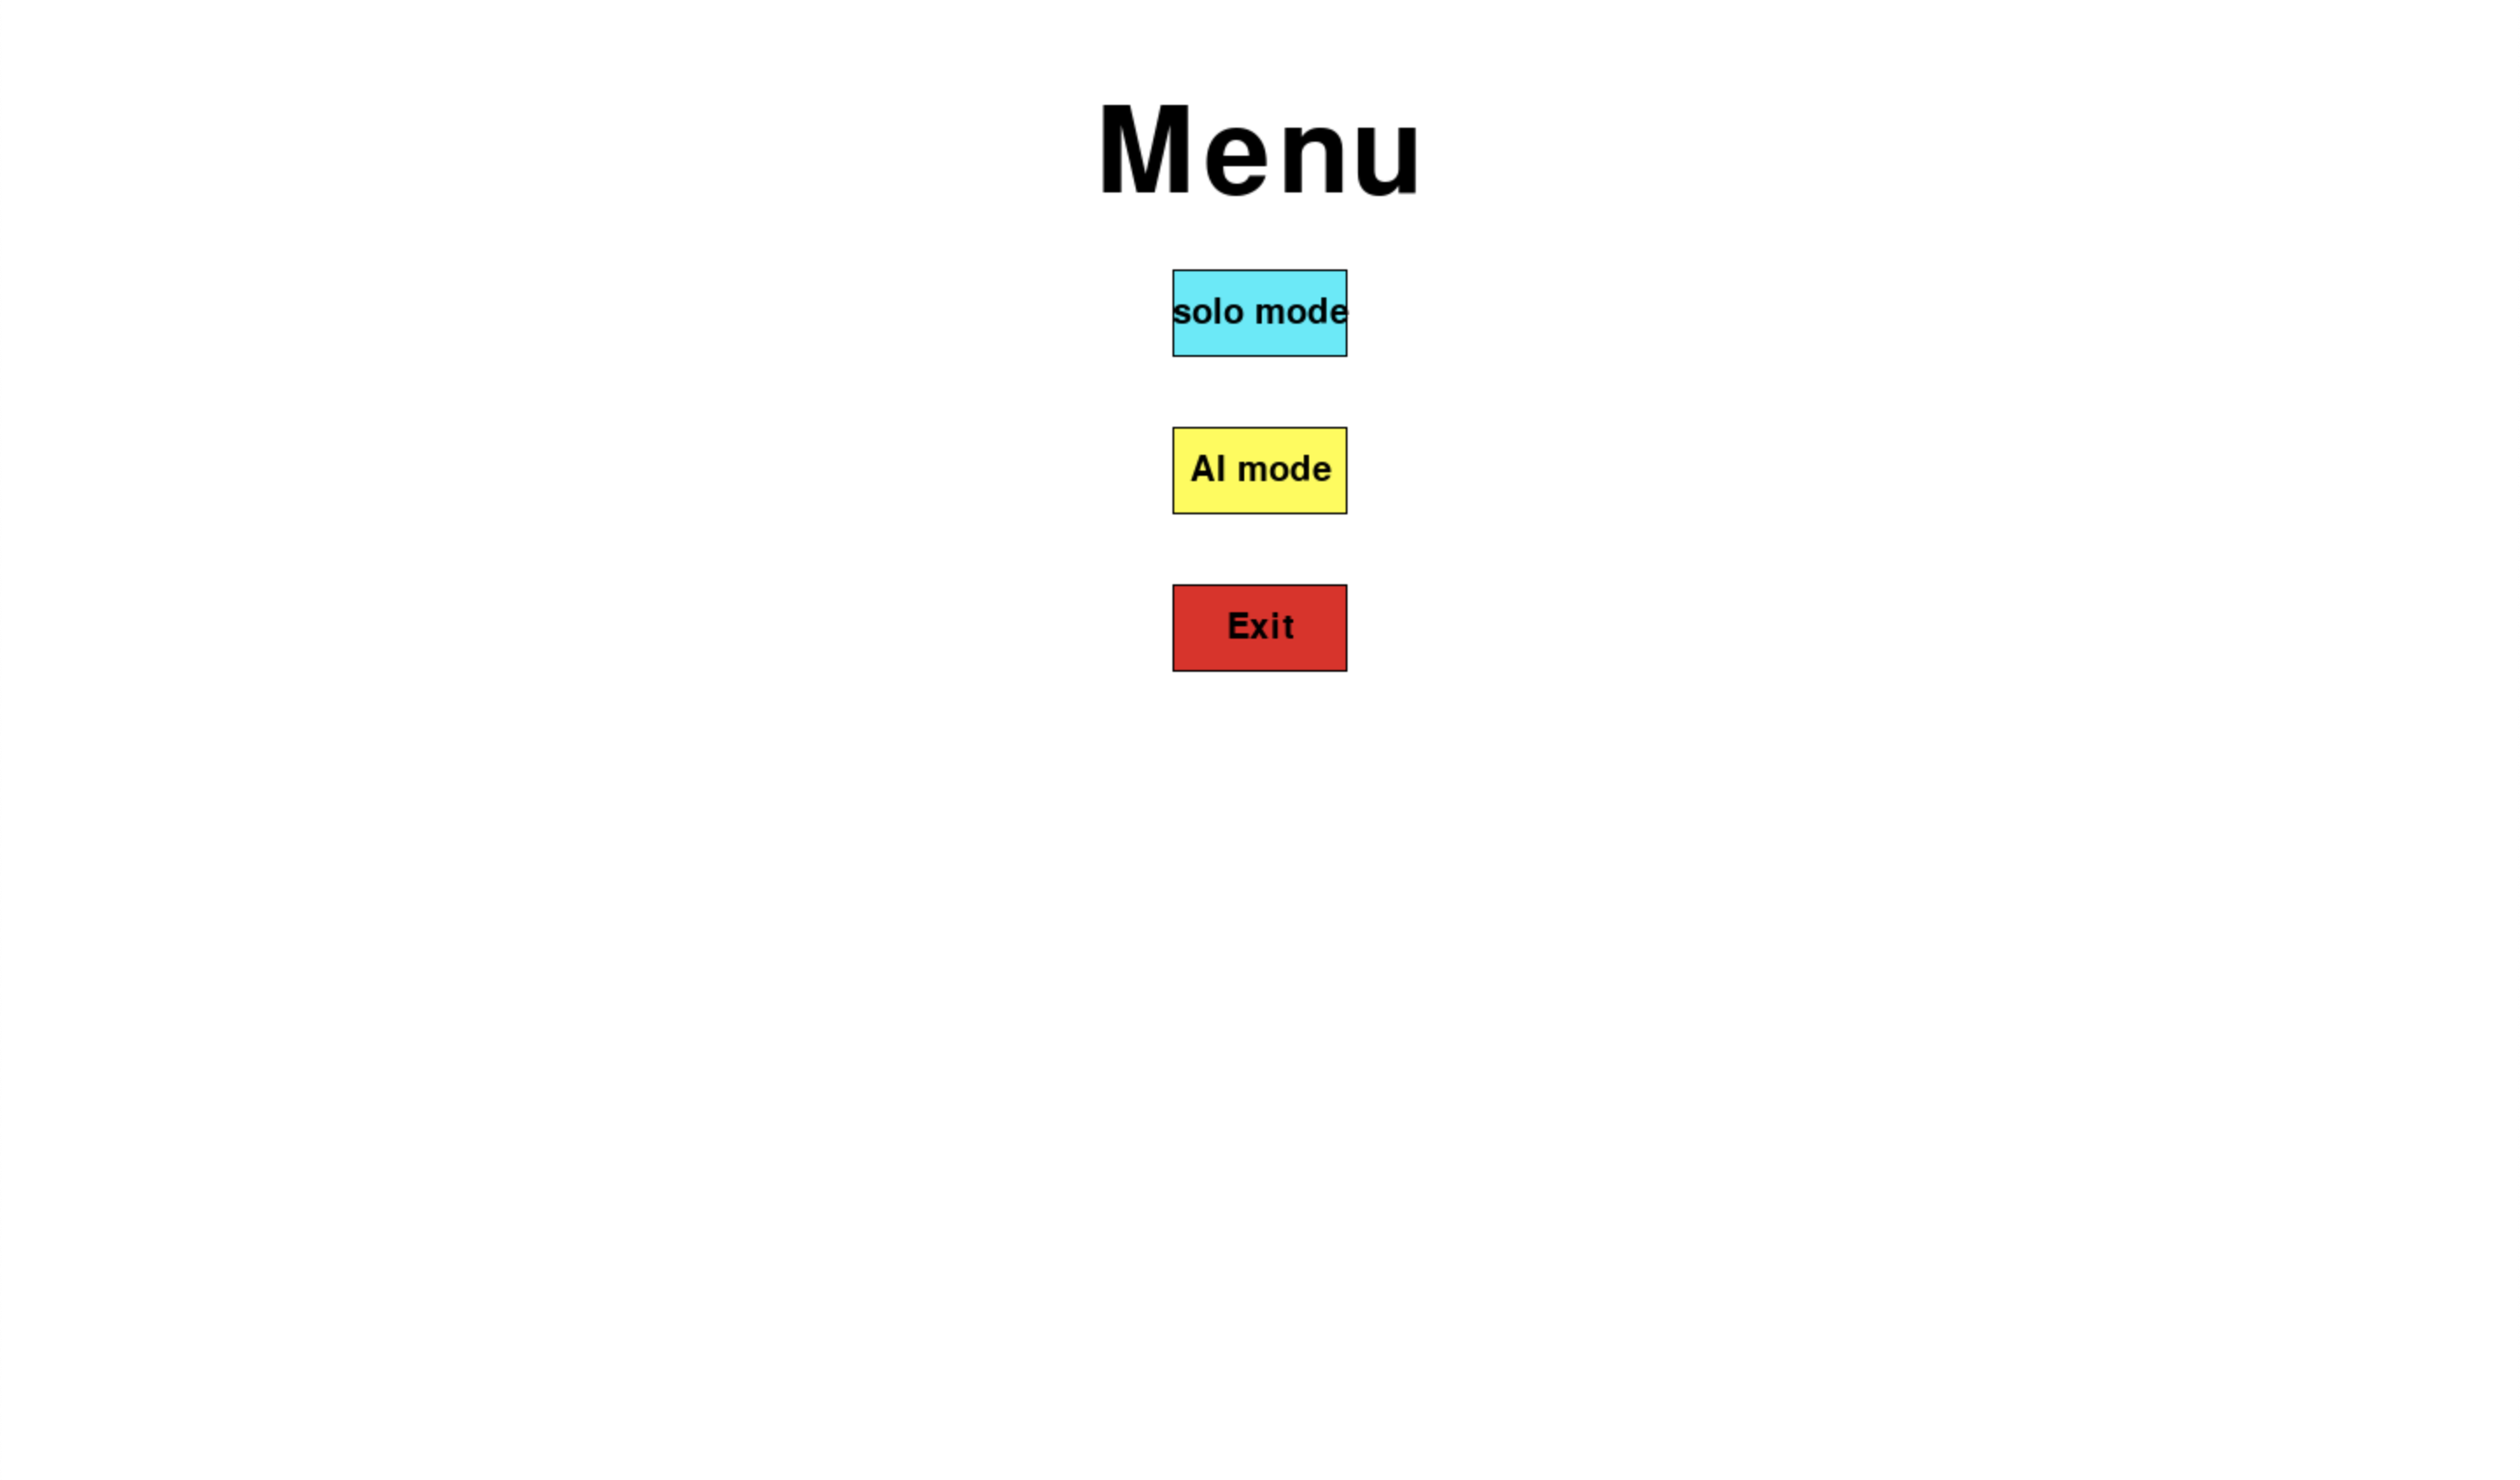
\includegraphics[scale = 0.13]{Menu Screen.png}}
    \caption{Screenshot of Triste - Menu}
    \label{fig:Display}
\end{figure} \\

\item Solo Mode: \\
When the user clicks the “Solo Mode” option, they will be brought to the following screen showing a basic game of Tetris. To control the movement of the Tetrominoes, the user can use the Left and Right arrow keys to move the game pieces, the Up arrow key to rotate the game pieces, the Down arrow key to drag the game pieces down slowly, and the Spacebar to drop the game pieces.
\begin{figure}[htbp]
\centering
    \fbox{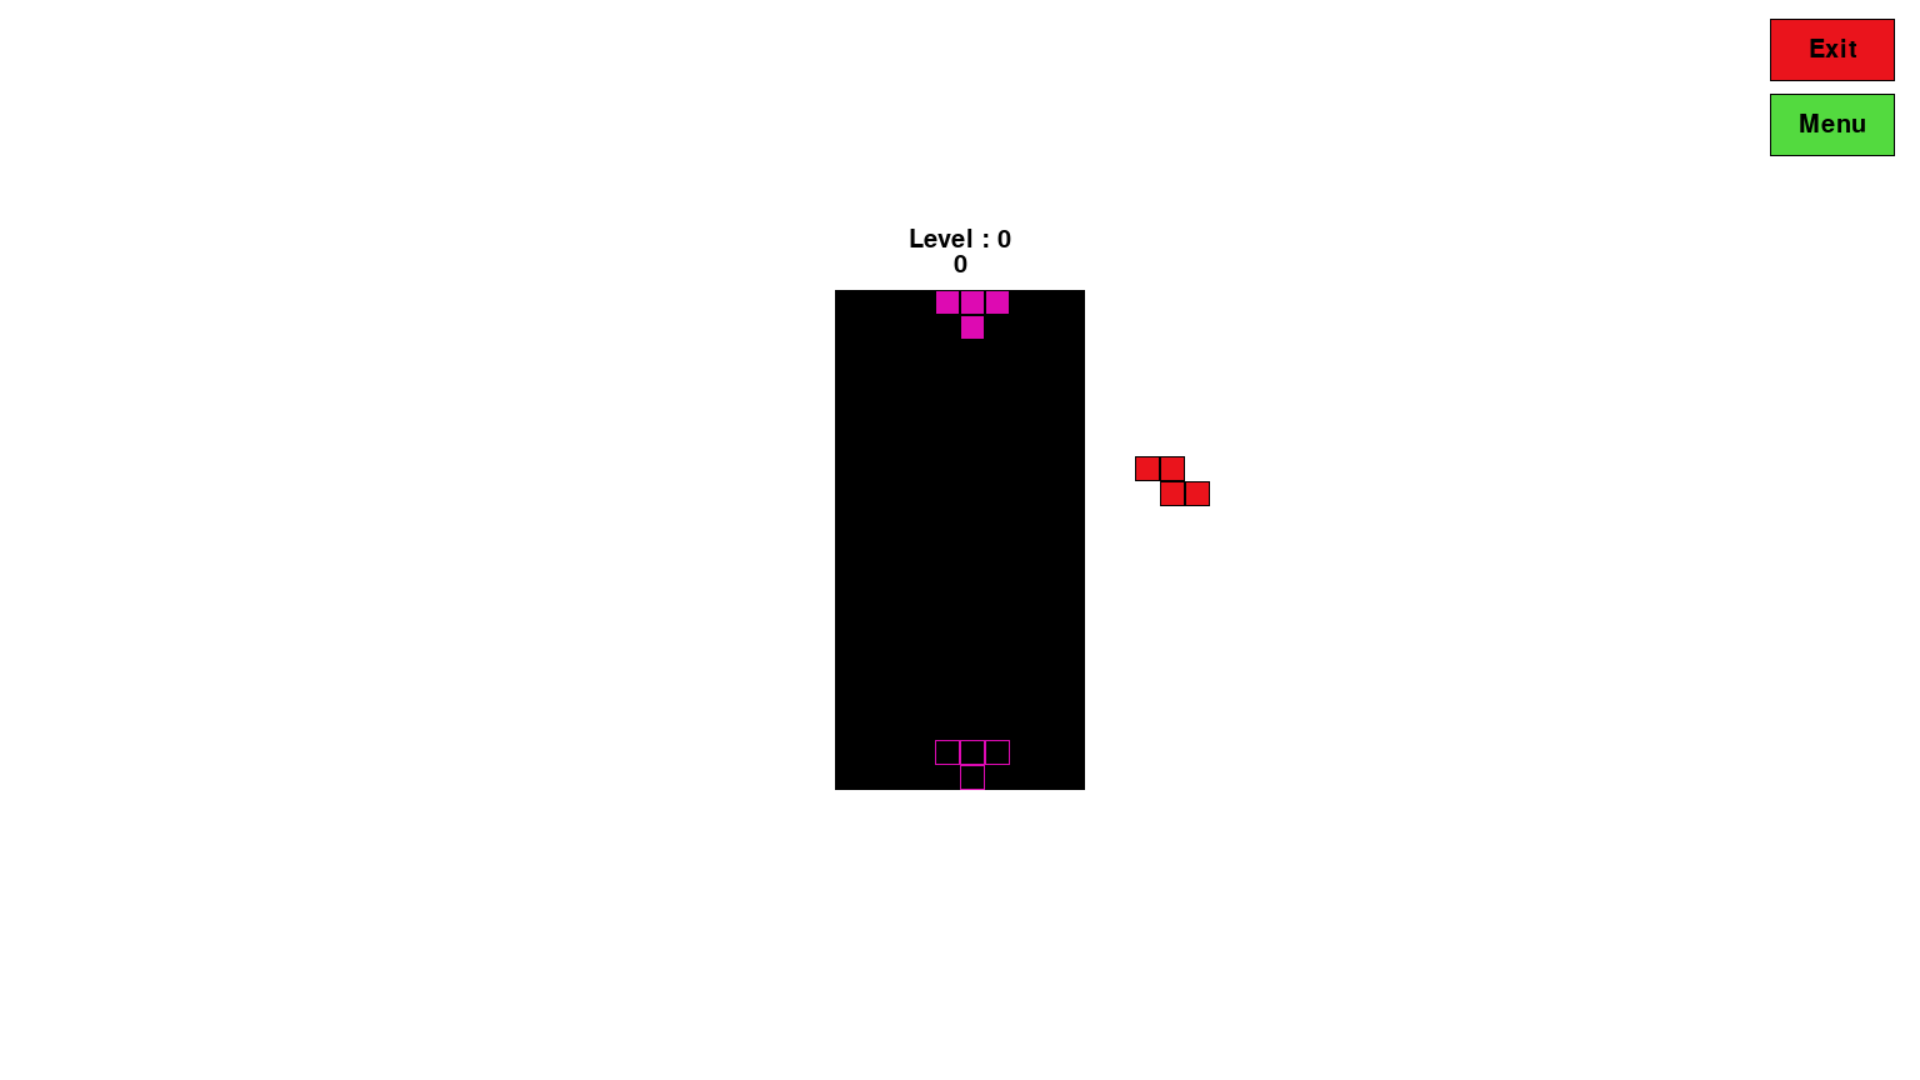
\includegraphics[scale = 0.13]{Solo Screen.png}}
    \caption{Screenshot of Triste - Solo Mode}
    \label{fig:Display}
\end{figure} \\
\vspace{20pt}

\item AI Mode: \\
When the user clicks the “AI Mode” option, the user will be brought to a screen exactly like the screen displayed in Solo Mode, but the AI will do all of the work to play the game until the limit is reached and the Game Over screen is displayed.
\begin{figure}[htbp]
\centering
    \fbox{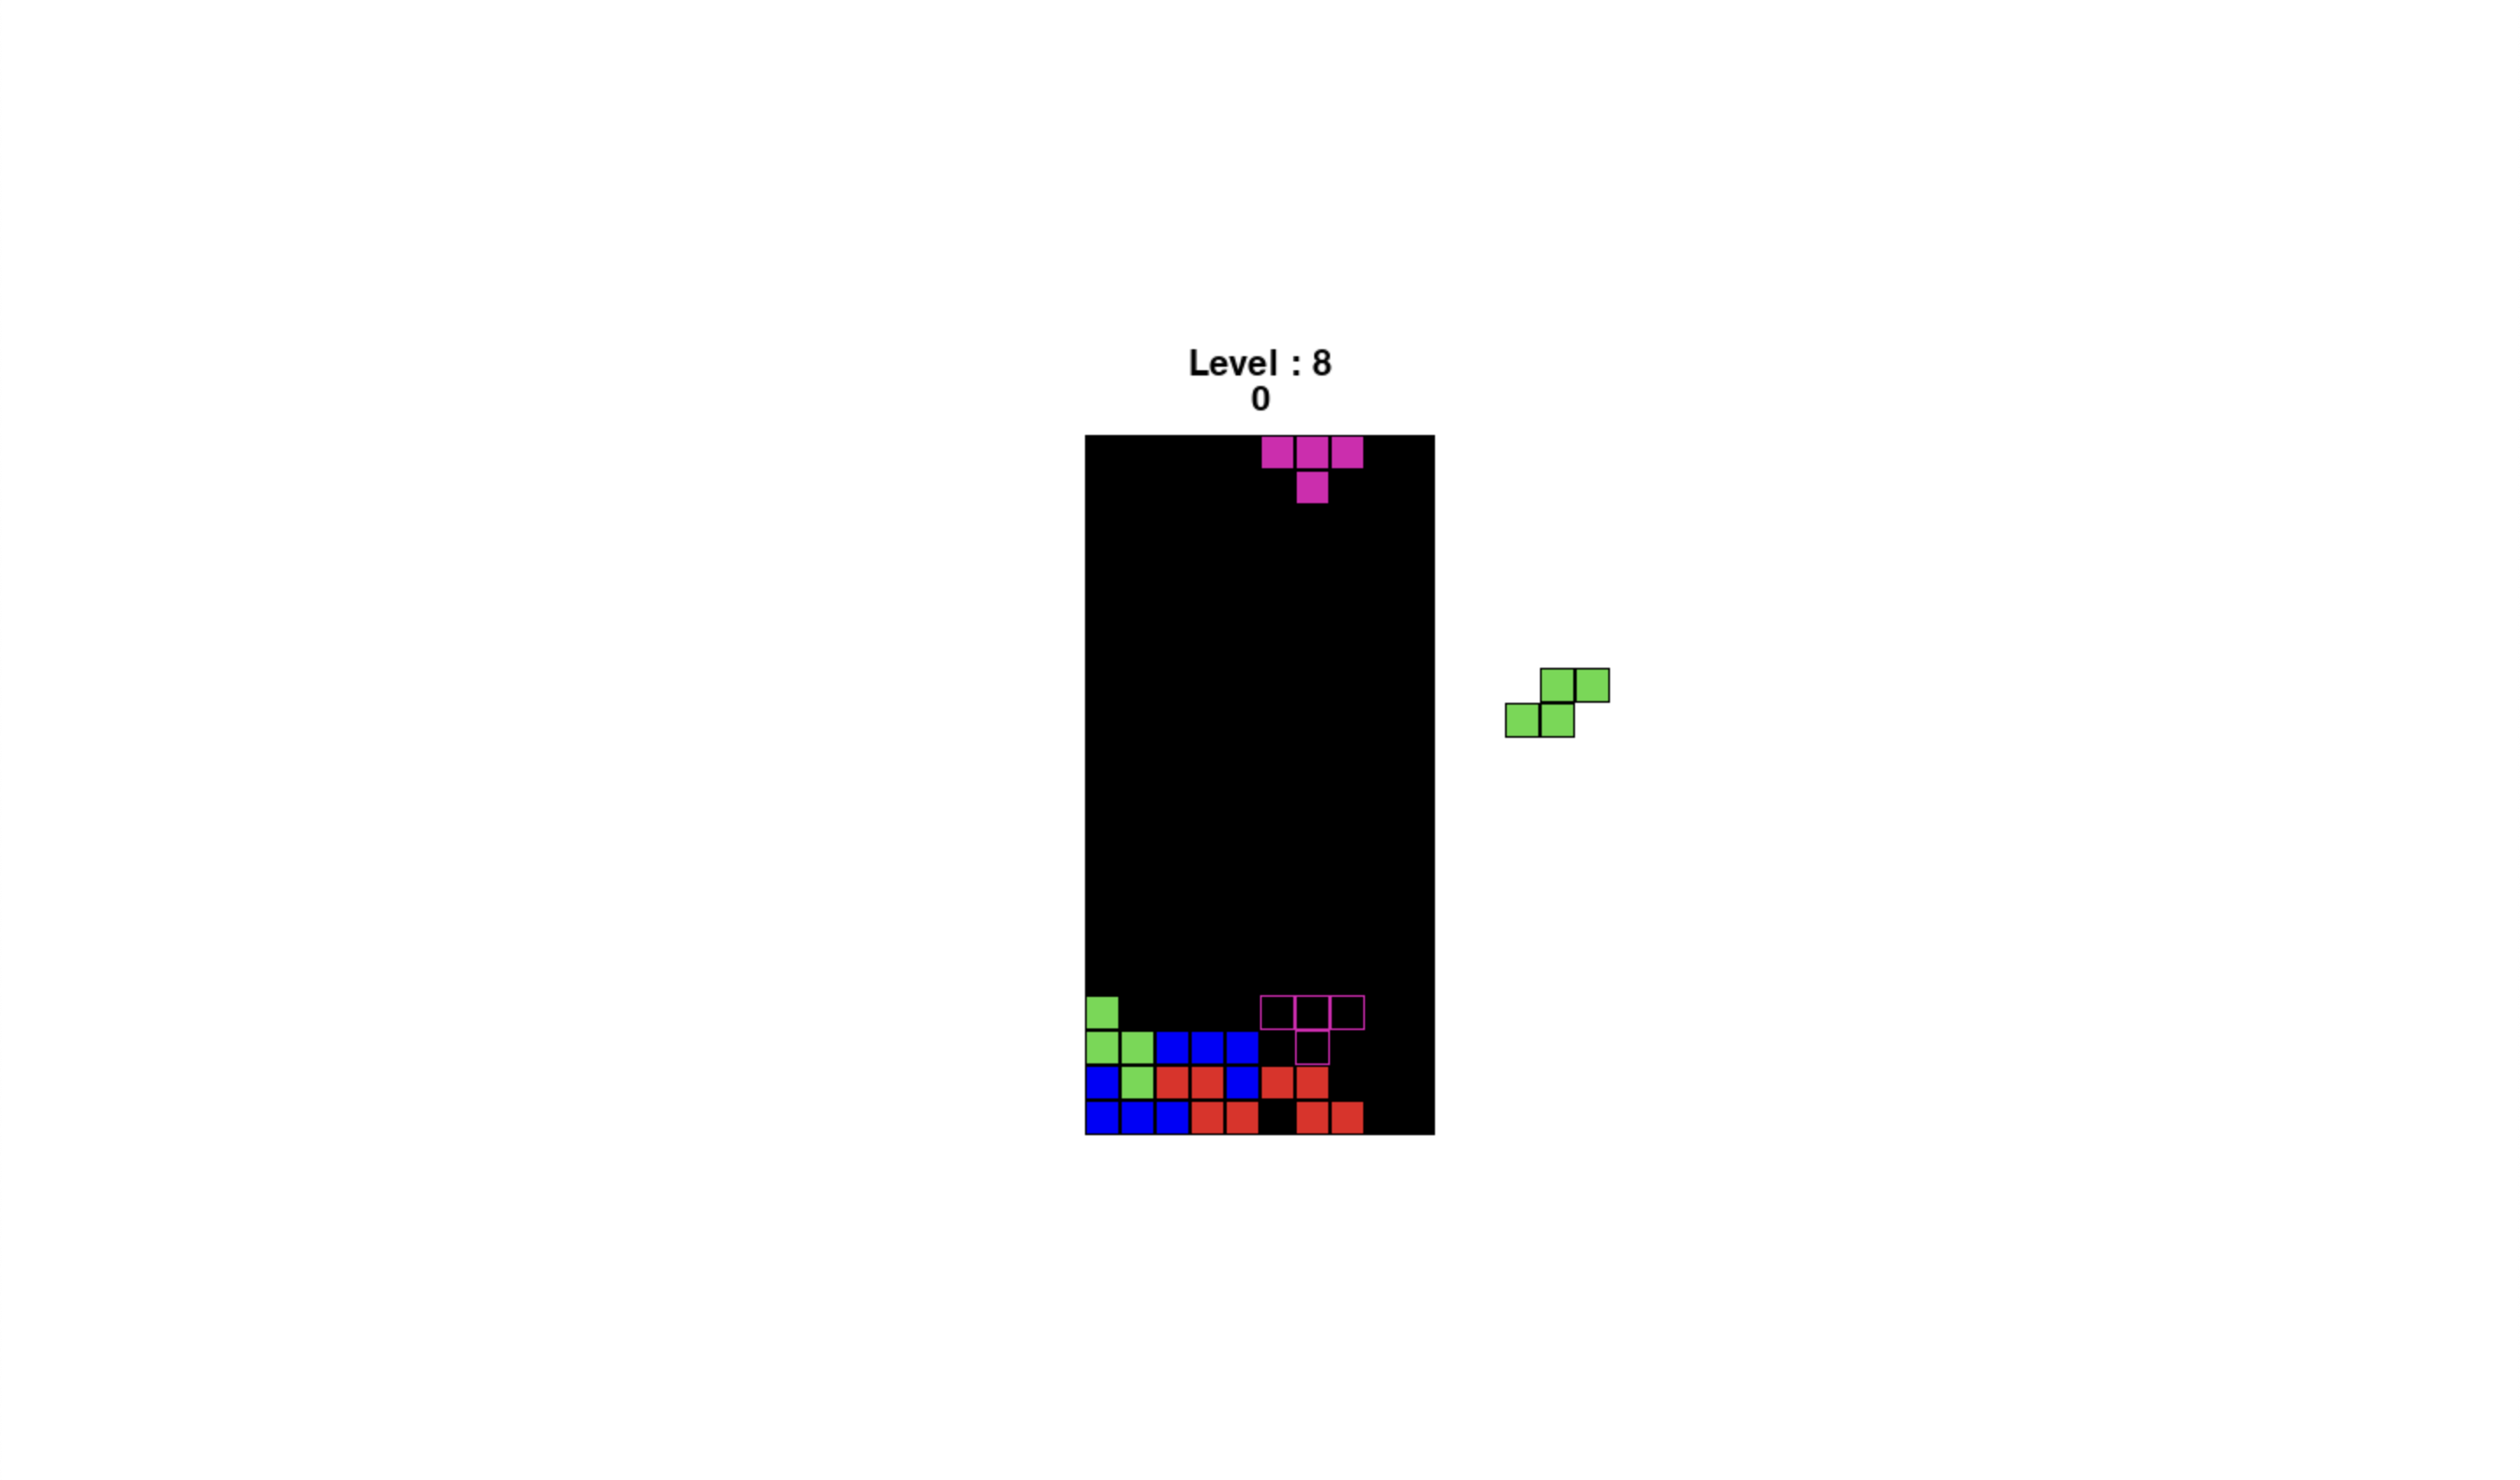
\includegraphics[scale = 0.13]{AI Screen.png}}
    \caption{Screenshot of Triste - AI Mode}
    \label{fig:Display}
\end{figure} \\

\item Game Over: \\
Regardless of whichever mode the user selects, when the game has reached its limit and no more Tetrominoes can be placed, the Game Over screen will be displayed. From this screen, the user will see their score for the current game, and the best score achieved from the game. Then, the user can chose to either restart in the mode that was previously selected, return to the main menu and select a different mode, or exit the game. When the User exits the game, the window is closed.
\begin{figure}[htbp]
\centering
    \fbox{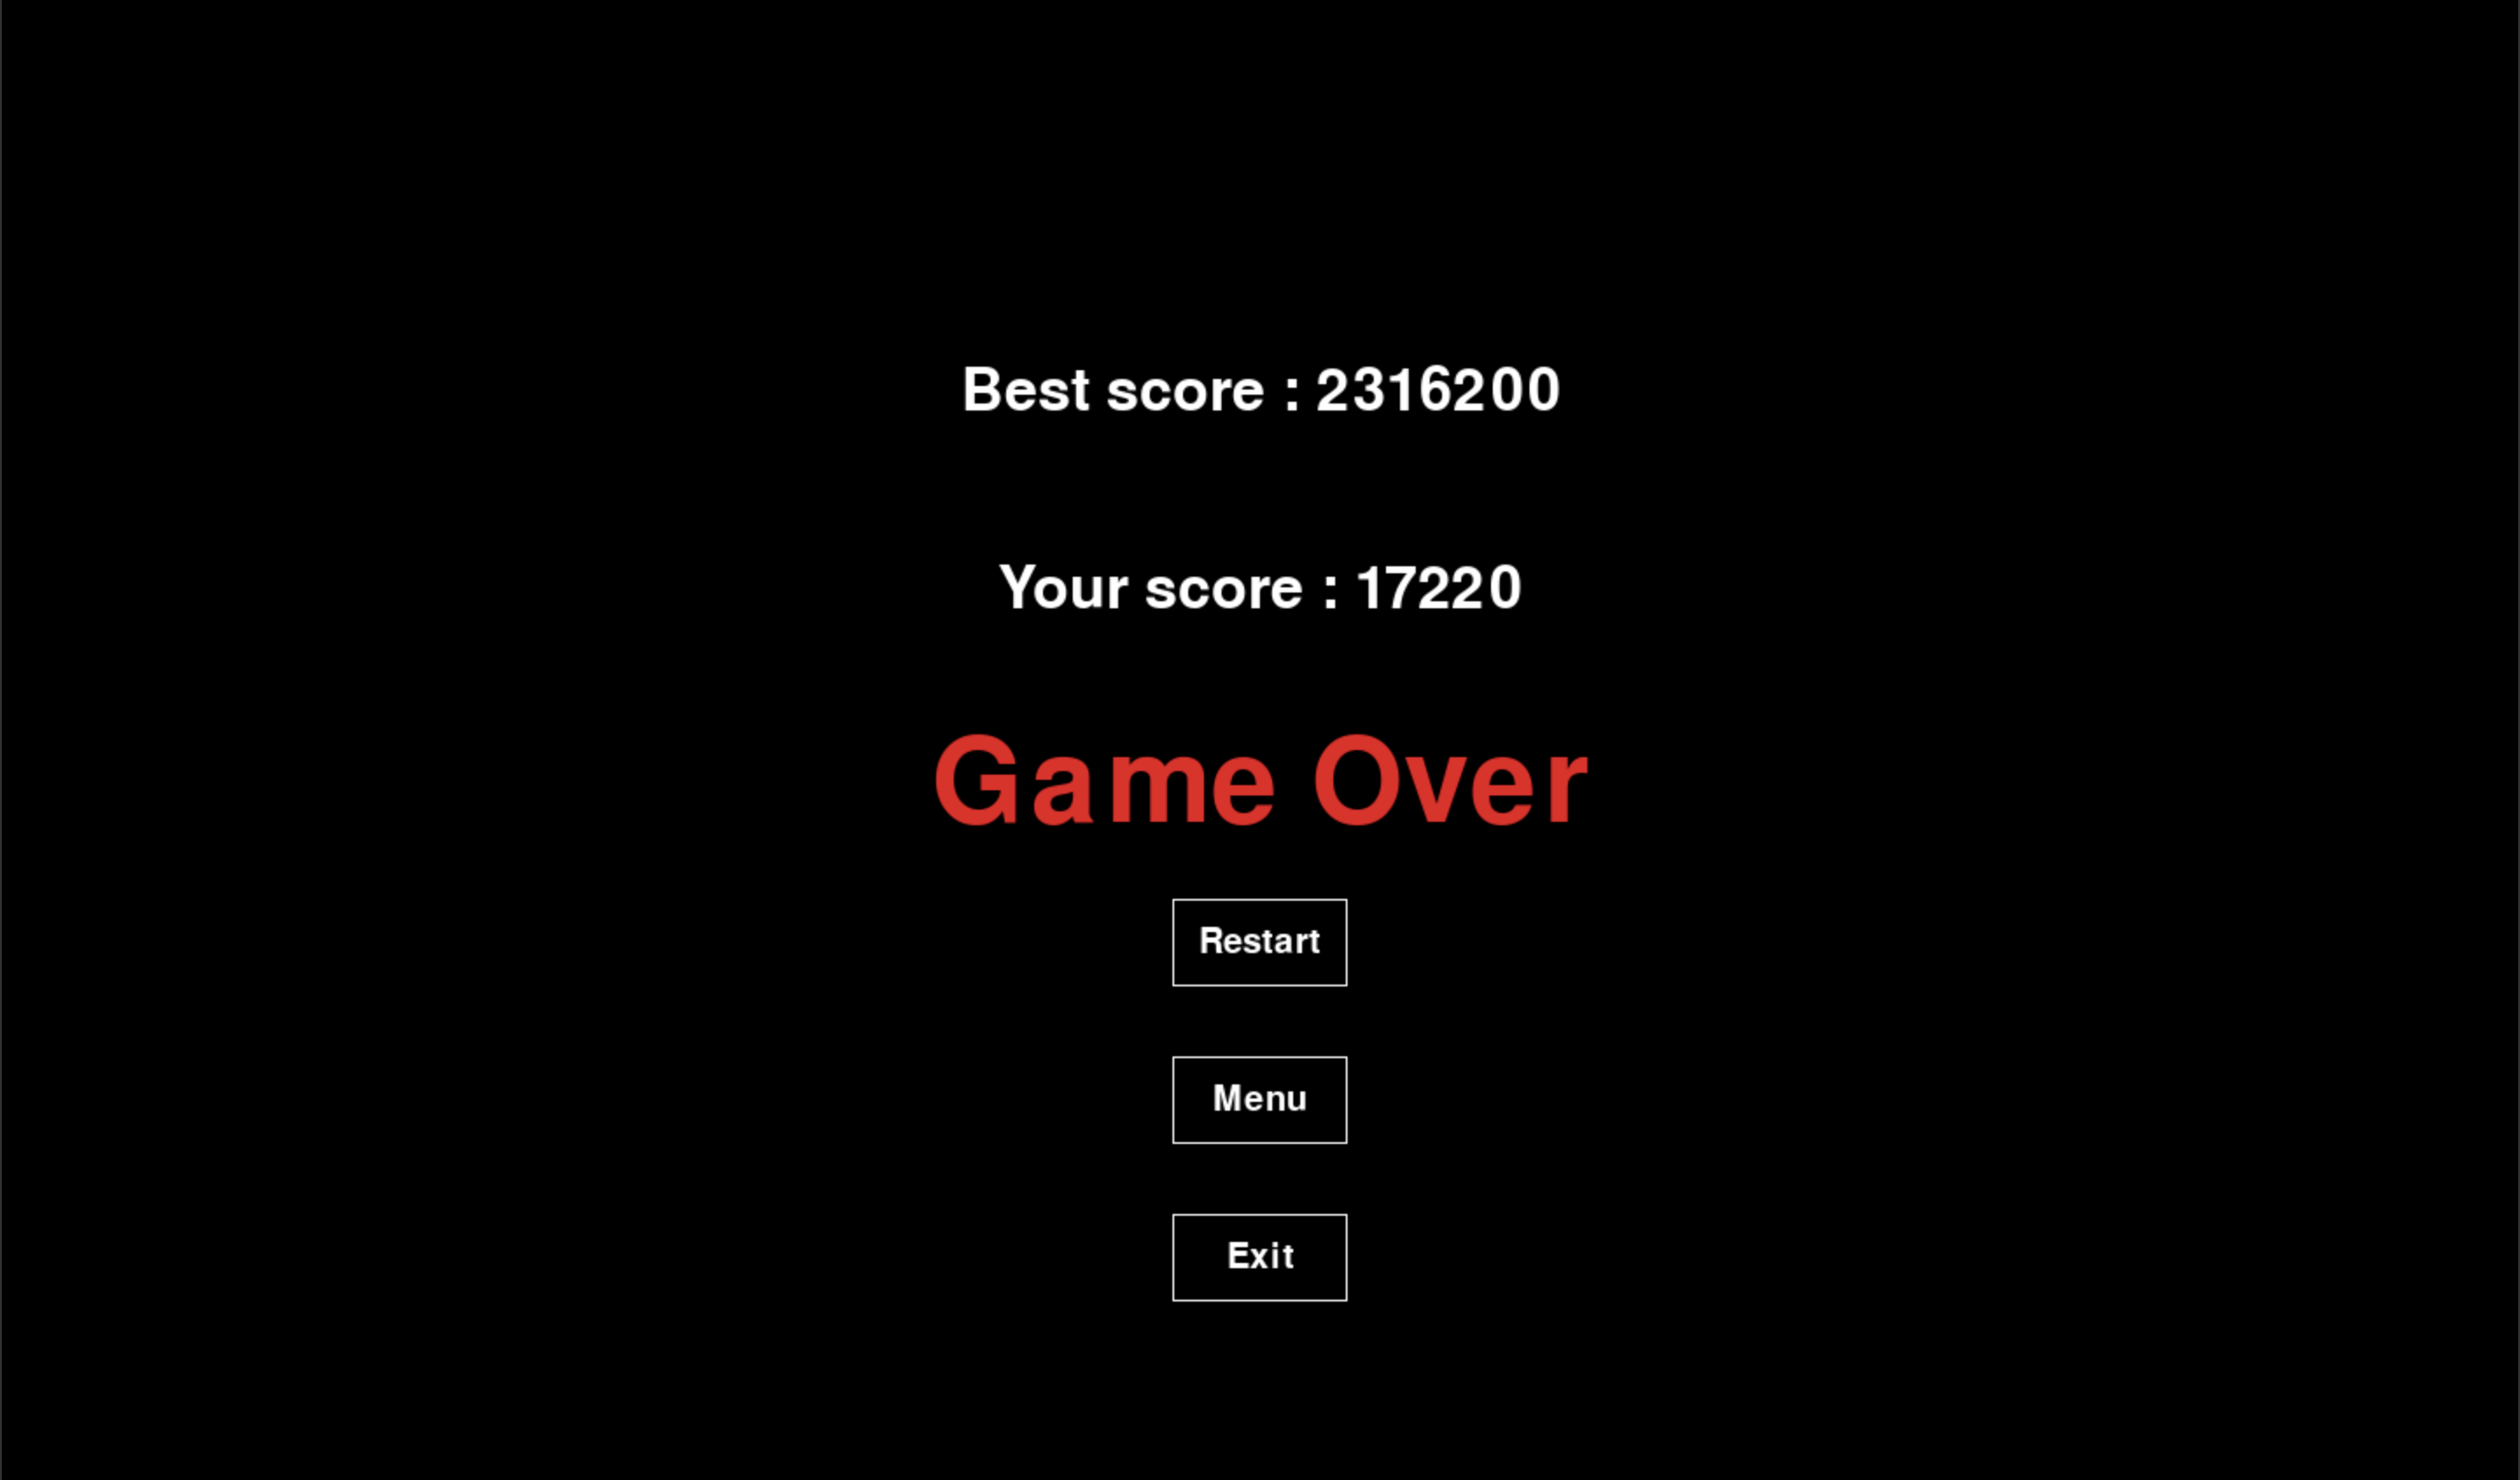
\includegraphics[scale= 0.13]{Game Over.png}}
    \caption{Screenshot of Triste - Game Over}
    \label{fig:Display}
\end{figure} \\
\end{enumerate}

\begin{thebibliography}{00}
\bibitem{b1} Code Bullet, "I Created An A.I. to DESTROY Tetris", YouTube, [Online]. Available : \url{https://youtu.be/QOJfyp0KMmM?si=dKykHlZGzpcrUu4L} [Accessed Oct. 7, 2023]

\bibitem{b2} Greg Cannon, "AI BREAKS NES TETRIS! - 102 MILLION and level 237", YouTube, [Online]. Available : \url{https://youtu.be/l_KY_EwZEVA?si=QNukpvk903yk_8xA} [Accessed Oct. 7, 2023]

\bibitem{b3} "Tetris ai", Github, [Online]. Available : \url{https://github.com/search?q=tetrisai&type=repositories} [Accessed Oct. 7, 2023]

\bibitem{b4} "Pygame Front Page", Pygame, [Online]. Available : \url{https://www.pygame.org/docs/} [Accessed Oct. 10, 2023]

\bibitem{b5} "PyTorch Front Page", PyTorch, [Online]. Available : \url{https://pytorch.org/} [Accessed Oct. 10, 2023]

\bibitem{b6} "random — Generate pseudo-random numbers", Python Docs, [Online]. Available : \url{https://docs.python.org/3/library/random.html} [Accessed Oct. 10, 2023]



\end{thebibliography}



\end{document}